\appendix
\renewcommand{\thesection}{\Roman{section}}    %change le mode de numérotation
\section{Compte-rendu des rencontres avec une institutrice et une logopède \label{annexeInterview}}
\subsection{Rencontre avec une institutrice : Odile Paveau}
J'ai rencontré Odile Paveau dans sa classe de primaire le 16 décembre 2014 dans la classe de primaire où elle enseigne, à l'école des Bruyères de Louvain-La-Neuve. \\

Elle m'a expliqué ce qu'elle, en temps qu'institutrice primaire, utilise comme méthodes pour enseigner la lecture. Elle m'a de même montré les outils utilisés à l'école afin de faciliter l'enseignement et l'apprentissage chez les enfants, ainsi que "l'ordre" dans lequel ceux-ci sont utilisés. Par exemple, un des premiers acquis de l'enfant sera toujours de savoir lire et écrire son prénom, puis celui de ses camarades de classe.\\

Elle m'a tout d'abord parlé des différentes méthodes d'apprentissage qui peuvent être utilisées. Parmi celles-ci, on retrouve :
\begin{itemize}
\item La méthode globale
\item La méthode syllabique
\item La méthode naturelle\\
\end{itemize}

La méthode globale consiste à apprendre à lire à partir du mot en entier. Le but de cet méthode est \textit{"de faire acquérir à l'élève une stratégie de déchiffrage des mots, voire des phrases, en tant qu'image visuelle indivisible"}\footnote{Citation tirée de l'article \textit{Méthode globale}, http://fr.wikipedia.org/wiki/Méthode\_globale}. En pratique, cela signifie que l'enfant, la première fois qu'il rencontre le mot, est invité à le deviner. Celui-ci mémorisera alors le mot en le rencontrant plusieurs fois dans des contextes différents (chansons, petites histoires, poèmes, ...). Le mot est dès lors associé à une idée, d'où le fait que cette méthode est qualifiée d'\textit{idéovisuelle}.\\

La méthode syllabique, par opposition à la méthode globale, part des sons que forment les lettres et les syllabes afin de construire le mot. Celle-ci relie la phonétique des lettres avec l'alphabet afin de construire tout d'abord les syllabes, puis d'assembler ces dernières pour créer les mots. Cette méthode se base sur le décryptage progressif des phrases lues.\\

La méthode naturelle est quant à elle inspirée de la pédagogie Freinet. Cette dernière, mise au point par Célestin Freinet durant le siècle dernier, est fondée sur l'expression de la créativité des enfants. Il s'agit de donner à l'enfant un projet, qui lui sera utile dans son apprentissage, et qui prend en compte ses centres d'intérêts et le potentiel créatif et associatif de celui-ci. Du point de vue de l'apprentissage de la lecture, cette méthode implique de partir du sens des mots, afin de donner un sens à ce qui est appris. La collaboration de tout le groupe est nécessaire, et l'essai-erreur est appliqué. La pédagogie Freinet a d'abord été associée à la méthode globale. Cependant, son procédé différant dans la façon dont les mots sont appris, l'apprentissage de la lecture par cette pédagogie se nomme désormais méthode naturelle.\\

Odile m'a ensuite fait part des techniques utilisées par elle-même et ses collègues aux Bruyères. La lecture s'apprend tout d'abord sur des caractères imprimés en majuscules, puis en minuscules, et enfin avec la police de type écriture manuelle, appelée aussi \textit{Cursive}. Ils utilisent principalement la méthode syllabique et la méthode naturelle. Ils discriminent à la fois les mots de manière visuelle et auditive. Toujours dans l'exemple du premier acquis que représente le prénom, en début de première primaire, les prénoms des enfants sont classés sur un tableau selon le son par lequel ils commencent. Ensuite, ils observent comment s'écrit le son du début du prénom, ce qui leur apprend déjà de premières syllabes. Par exemple : Amélie commence par le son "A", qui s'écrit de la même manière, tandis qu'Hugo commence par le son "U" mais s'écrit "HU".\\

Durant la suite de l'apprentissage, le rapport au son reste très important pour l'enfant. Voici quelques exercices et outils qui sont proposés à l'école :
\begin{itemize}
\item Avec des lettres d'imprimerie disposées dans n'importe quel sens\footnote{Le fait de mettre les lettres droites, à l'envers, ou de côté permet d'entraîner l'enfant à différencier les caractères.}, l'institutrice donne un son, et il faut retrouver la lettre qui produit ce son.
\item Dans un petit texte, qui peut être écrit sur base d'une idée de l'enfant (par exemple "\textit{Marie aime la danse et les poupées}"), retrouver les sons déjà connus et les souligner en couleur. La couleur aide ici et à mémoriser, et à différencier.
\item Dans un texte, trouver le son qui revient le plus souvent. Cet exercice est une variante du précédent.
\item A partir d'un son, trouver des mots qui commencent par celui-ci, par exemple sous forme d'images pour ensuite voir comment s'écrit le mot. Au niveau supérieur, le son peut se trouver au milieu ou en fin de mot.
\item Comme outil, créer un dictionnaire \textit{référent}. Celui-ci reprend, pour chaque son (également les composés type \textit{au, ou, en, ...}) un dessin représentatif du son (par exemple une chouette pour le son \textit{ch}) ainsi qu'une liste des mots commençant par ce son.\\
\end{itemize}

Parmi les exemples ci-dessus, on constate que la méthode syllabique n'est pas la seule appliquée. En effet, on retrouve la méthode naturelle dans l'association avec les couleurs et les images. En effet, il est très important de faire sens pour l'enfant et de l'intéresser pour faciliter l'apprentissage. Ainsi, le faire travailler sur des sujets qui le concernent tels que son âge, ce qu'il aime, faire des phrases rigolotes, etc.\\

La méthode globale est aussi utilisée aux Bruyères, mais peu comparativement aux deux autres. Celle-ci est considérée comme plus lourde et moins efficace. Néanmoins, on retrouve son application dans des exercices de repérage d'un mot en particulier dans un texte, de chasse aux mots dans la classe, et quelques autres.\\

Lors des évaluations pour constater l'apprentissage de la classe, la méthode naturelle est la plus souvent utilisée, car c'est celle qui fait le plus appel à l'imagination de l'enfant. Comme outil, les instituteurs utilisent notamment les fichiers Freinet. Créés à partir de la pédagogie Freinet, ces fichiers sont composés d'images associées à des mots de différents niveaux. L'idée est d'associer un (ou plusieurs) mot(s) lu(s) à une (ou plusieurs) image(s), et de vérifier les capacités de lecture de l'enfant en lui proposant soit le même mot à retrouver dans une liste sur base d'une image semblable à la précédente, soit un mot différent sur base d'une image différente des deux précédentes, soit encore l'association d'un nouveau mot en complément avec celui lu précédemment, sous forme d'une phrase. Des exemples de fichiers se trouvent dans l'annexe \ref{annexeFreinet}. Ces fichiers existent également pour d'autres matières, comme les mathématiques.\\

Enfin, à l'école des Bruyères, l'enfant à toujours accès à une boîte à outils pour s'aider en cas de difficultés. Celle-ci est composée du dictionnaire référent, mais aussi de panneaux et d'affiches se trouvant un peu partout dans la classe. Ceux-ci rappellent les couleurs identifiants les sons, les images associées, les dessins des enfants représentant des mots, des symboles associés aux lettre (par exemple une montage double pour le M), etc. Mis à part ces outils, il est important de faire attention à l'ancrage gauche - droite correspondant au sens de la lecture. Certains enfants ont du mal avec cette notion.

\subsection{Rencontre avec une logopède : Laurence Henrion}
J'ai rencontré Laurence Henrion le 19 janvier 2015. Elle a accepté de me recevoir dans le cabinet où elle exerce son activité de logopède pour répondre à mes questions.\\

Elle a commencé par m'expliquer qu'il existe plusieurs méthodes pour apprendre à l'enfant à lire. L'idéal, cependant, est de commencer à lui inculquer les bases de la lecture vers 3 ou 4 ans. En effet, ceci permet d'optimiser ses compétences par la suite. La méthode proposant de commencer l'apprentissage si tôt s'appelle \textit{Montessori}. Celle-ci part du principe qu'il existe une conscience phonologique fort présente chez l'enfant. Celui-ci apprend beaucoup à l'aide de rimes, de comptines, etc. C'est-à-dire à l'aide de sons. Ceci rejoint ce qui m'avait déjà été dit par Odile à propos de la méthode syllabique : il est important de se baser sur le son que fait la lettre seule, ou le groupe de lettres, et non le nom qui lui est donné, car ce dernier apporte des confusions.\\

De plus, elle a insisté sur le point suivant : pour apprendre à lire, l'enfant doit déjà maîtriser un certain vocabulaire à l'oral. Dès lors, si le vocabulaire de base n'est pas acquis, l'enfant ne sera pas capable de comprendre ce qu'il lit. Les premiers mots et textes seront dont composés de vocabulaire basique, pas de mots compliqués et peu fréquents, tels que \textit{narval}, \textit{okapi}, etc. \\

En tant que logopède, elle travaille essentiellement sur base des sons pour aider l'enfant à discriminer les lettres qui posent problème. Elle ne s'est pas étendue sur son travail, ceci n'étant pas le but de la rencontre, mais m'a  expliqué ce qu'elle considérait comme la technique la plus porteuse de résultats. Cette technique se base sur la méthode syllabique et Montessori, et rejoint en beaucoup de points celle appliquée par les instituteurs de l'école de Bruyères expliquée dans le point précédent. Parmi les points communs avec ce qui m'avait été expliqué précédemment, on trouve :
\begin{itemize}
\item La sélection d'un mot contenant un son entendu précédemment parmi plusieurs choix.
\item Choisir une lettre qui produit le son prononcé. Ici, Laurence Henrion m'a spécifié que la lettre importait peut tant que le son était correct. Par exemple, pour le son \textit{sss}, l'enfant peut choisir aussi bien le \textit{s} que le \textit{c} ou le \textit{ç.}
\item Relier un mot ou un son à une image.
\item Associer les sons et les lettres à des couleurs qui leur seront spécifiques. Au départ, il peut simplement s'agir de donner par exemple les voyelles en rouge et les consonnes en bleu.\\
\end{itemize}

Laurence Henrion travaille avec les enfants essentiellement avec des applications sur son iPad. Elle était donc de bon conseil pour me renseigner sur ce qu'elle considère qu'il manque à ces applications, et sur les erreurs à ne pas produire. Elle m'a dit que sur iPad, elle trouve suffisamment d'applications spécialisées (peu toutefois reprenant plusieurs exercices), mais qu'il lui semble qu'il y a un manque de ce côté sur Android, ce pourquoi elle travaille sur iPad. Ceci m'a bien évidemment conforté dans mon choix.\\

La majorité applications présentes sur l'iPad ont été créés par un spécialiste orthophoniste (appelation d'un logopède en France) : Emmanuel Crombez. Celui-ci réalise des applications pour iPad, iPhone et Mac sous le nom \textit{ABC Applications}. Celles-ci sont destinées à aider les enfants dans leur apprentissage général et dans leurs difficultés : lecture, écriture, mathématiques, etc. Parmi ces jeux, on peut trouver\footnote{Liste complète sur le site d'Emmanuel Crombez : \url{http://abc-applications.com/ipad.html}.} :
\begin{itemize}
\item \textit{Anagrammes}. L'enfant doit retrouver des mots dont les lettres ont été mélangées. Au besoin, il peut s'aider en écoutant le mot qu'il doit reconstituer.
\item \textit{Nuages de mots}. Cet exercice propose à l'enfant de retrouver le genre et le nombre des mots affichés en "nuages". Quel mot est masculin, ou féminin ? Est-ce singulier ou pluriel ? Le jeu entraîne à la lecture mais aussi au classement. Ce jeu existe aussi sous la forme \textit{Nuages de lettres}, adapté aux enfants de maternelle pour apprendre à reconnaître les lettres.
\item \textit{Mémo des mots}. Ce jeu se présente sous la forme du bien connu \textit{Memory}. La différence étant qu'ici des mots sont utilisés à la place des images.
\textit{Etc.}\\

\end{itemize}
Le gros avantage des applications d'Emmanuel Crombez est qu'elles sont créés par une personne maîtrisant les processus d'apprentissage de l'enfant. De ce fait, il a pu optimiser l'interface afin d'éviter trop de distraction ou de difficultés. Sur cette base, Laurence Henrion m'a conseillé de ne pas inclure trop d'éléments graphiques et de garder un design simple et épuré. Trop d'objets sur l'écran c'est prendre le risque que l'enfant soit distrait et ne se concentre pas sur ce qui est requis, donc perdre en efficacité. Par ailleurs, elle m'a conseillé d'utiliser la police \textit{OpenDyslexic} pour mon application. Elle a pu tester cette police via les jeux de \textit{ABC Applications}. \textit{OpenDyslexic} est une police open source conçue pour faciliter la lecture chez les personnes dyslexiques en accentuant certaines parties des lettres. Dans le cas où cette police n'aurait pas été disponible, une police sans serif type \textit{Verdana} aurait convenu. Les polices sans serif sont plus faciles à déchiffrer, les pattes des lettres avec serif encombrant la vue.\\

Un autre exercice, indépendant de ceux précités, et pour lequel Laurence Henrion portait grand intérêt c'est la \textit{lecture flash}. Cet exercice consiste à mémoriser un mot (ou une phrase affiché) plus ou moins rapidement à l'écran, pour ensuite le réécrire correctement. Dans le cas présent, l'orthographe est travaillée en plus de la lecture. Ce sont deux matières très liées. Un jeu de lecture flash doit idéalement :
\begin{itemize}
\item avoir un temps réglable d'affichage selon le niveau de l'enfant
\item insister sur l'importance de la mémorisation
\item faire attention au sens de la lecture
\end{itemize}
En plus de cela, l'exercice peut être amélioré grâce à :
\begin{itemize}
\item l'affichage de mots personnalisés en fonction des centres d'intérêt de l'enfant
\item la lecture effectuée avec un mot, et la réécriture sous la forme d'une image à choisir\\
\end{itemize}

Enfin, j'ai également reçu comme conseil d'utiliser le VOB (Vocabulaire Orthographique de Base) pour les exercices que je mettrais en place dans l'application. Il s'agit de la liste officielle en Belgique des mots qui doivent être connus et maîtrisés par les enfants à la fin de chaque cycle de primaire.


\newpage
\section{Exemples de fiches Freinet}
\label{annexeFreinet}
\begin{center}
\begin{figure}[h]
   \begin{minipage}[c]{.46\linewidth}
      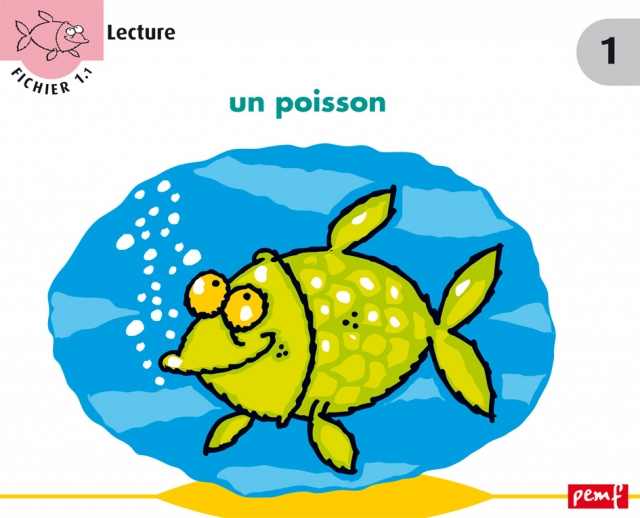
\includegraphics[width=7cm]{img/GSCP_f1recto.jpg}
   \end{minipage}  
   \begin{minipage}[c]{.46\linewidth}
      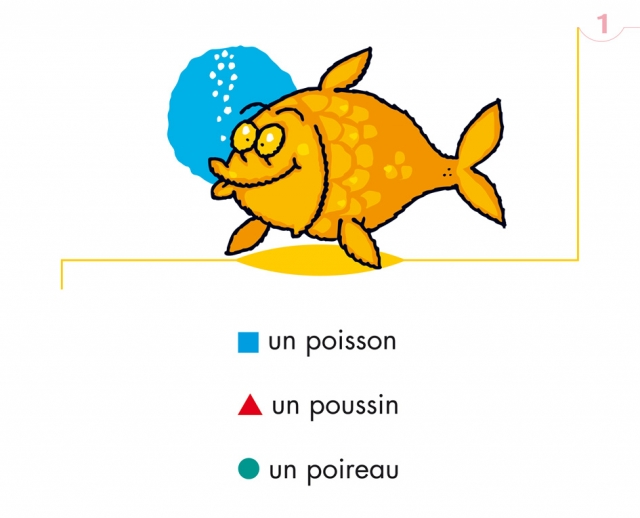
\includegraphics[width=7cm]{img/GSCP_f1verso.jpg}
   \end{minipage}
\end{figure}
\vline
\vline
\begin{figure}[h]
   \begin{minipage}[c]{.46\linewidth}
      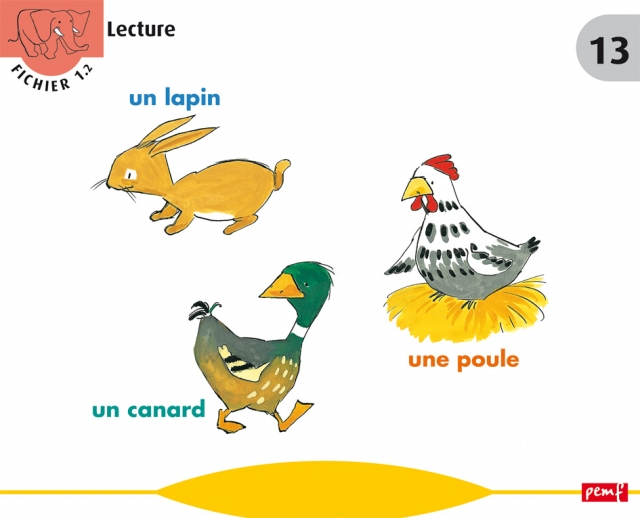
\includegraphics[width=7cm]{img/CP_niv2_f13recto.jpg}
   \end{minipage}  
   \begin{minipage}[c]{.46\linewidth}
      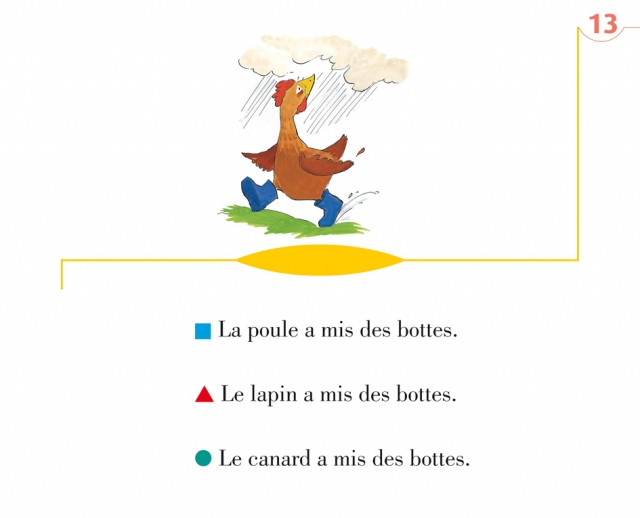
\includegraphics[width=7cm]{img/CP_niv2_f13verso.jpg}
   \end{minipage}
\end{figure}
\vline
\vline
\begin{figure}[h]
   \begin{minipage}[c]{.46\linewidth}
      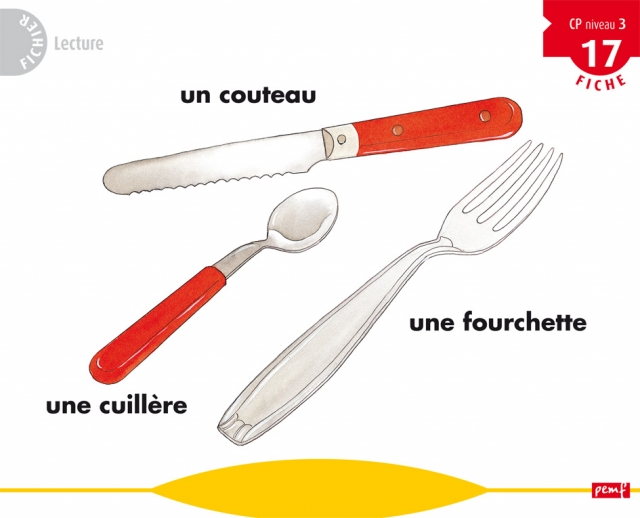
\includegraphics[width=7cm]{img/CP_niv3_f17recto.jpg}
   \end{minipage}  
   \begin{minipage}[c]{.46\linewidth}
      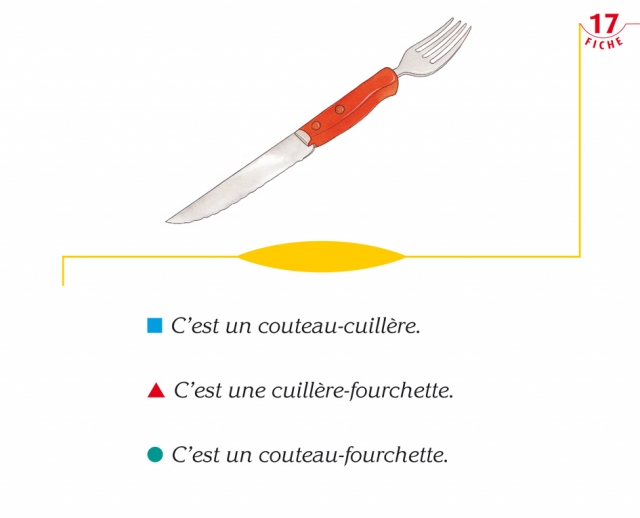
\includegraphics[width=7cm]{img/CP_niv3_f17verso.jpg}
   \end{minipage}
\end{figure}
\end{center}

\newpage
\section{VOB du cycle inférieur \label{listeVob}}
Voici la liste des mots devant être connus et maîtrisés par les enfants, téléchargée depuis \url{http://www.enseignons.be/upload/fondamental/francais/190607071618vob-degre-inferieur.pdf} le 26 janvier 2015.
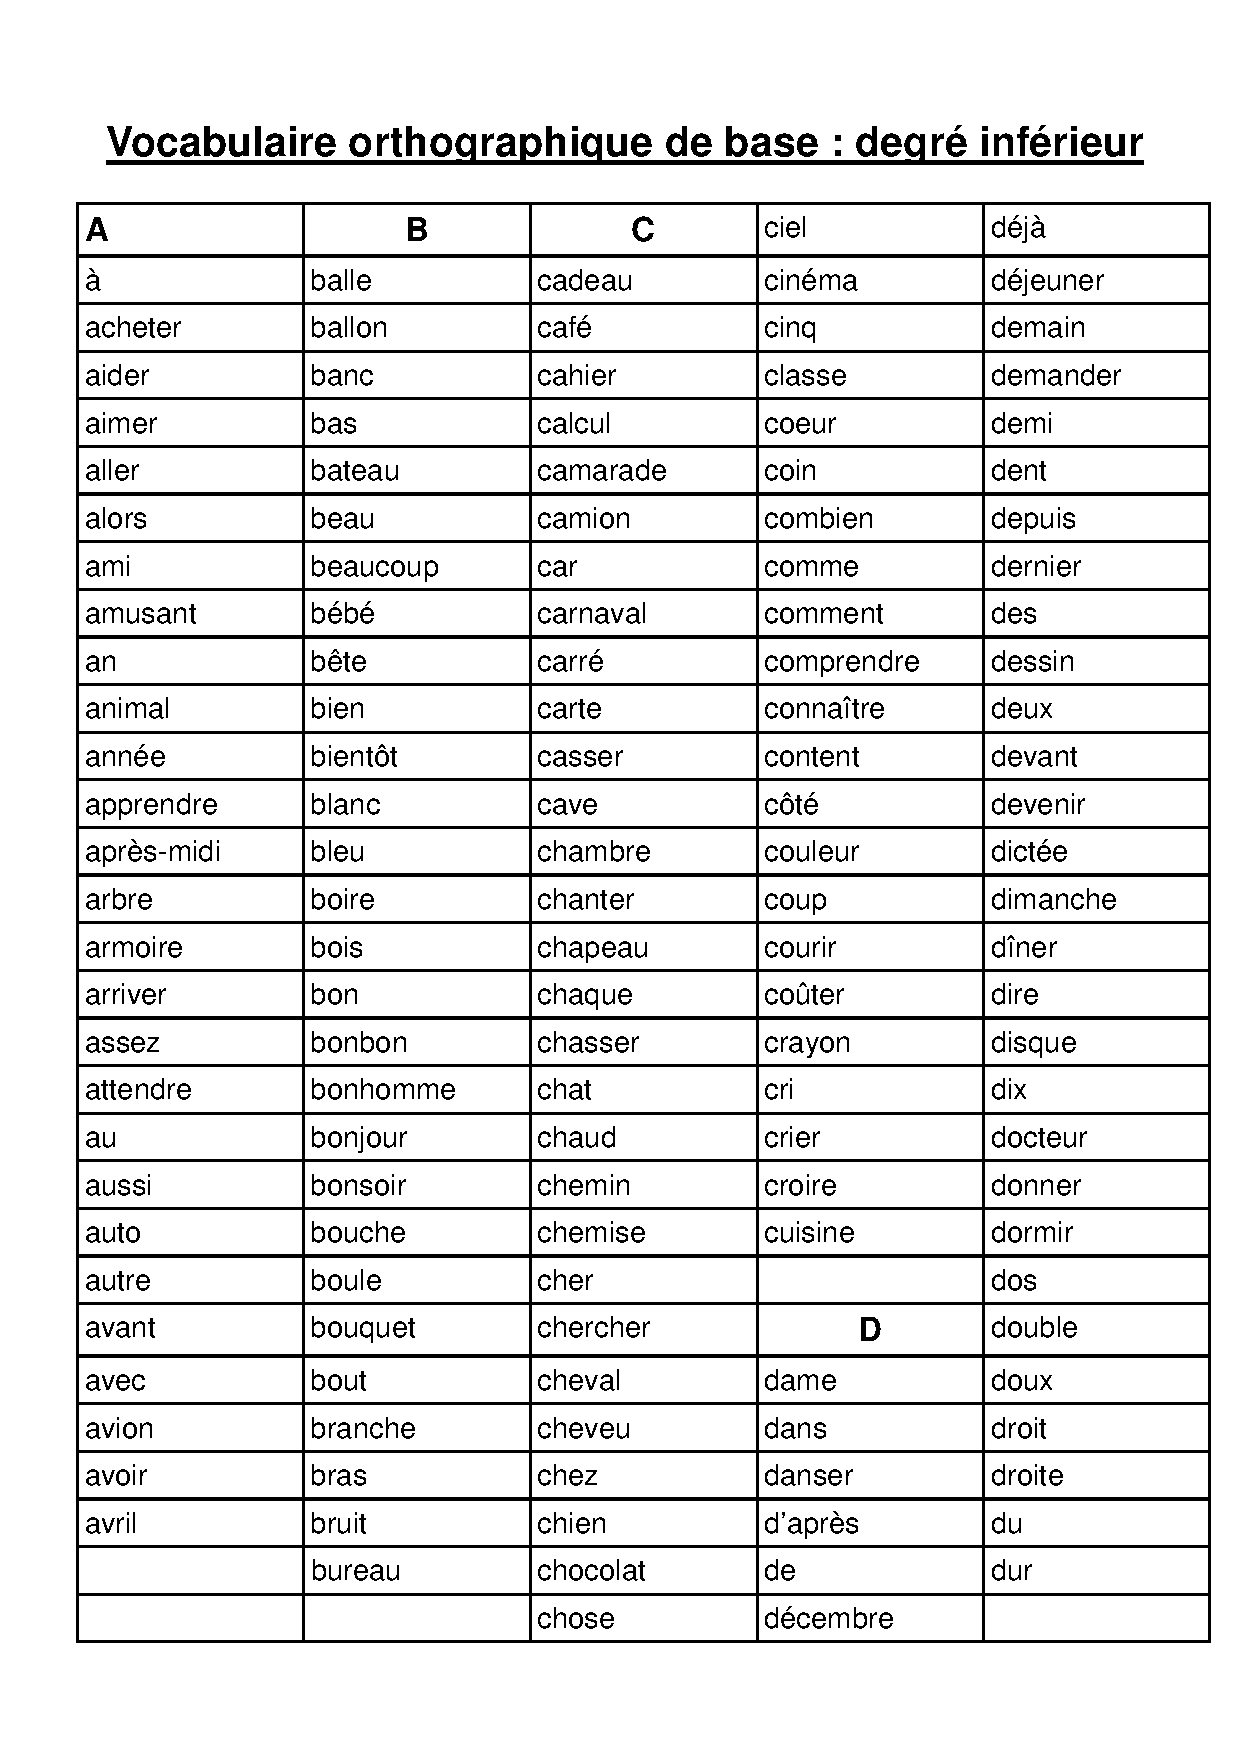
\includepdf[pages={1-4},scale=.9,pagecommand={}]{190607071618vob-degre-inferieur.pdf}

